\section{Instance Generation}

The instances are generated randomly \cite{bib:instances-CVRP}, \cite{bib:constrained-knapsack}, \cite{bib:grasp-and-tabu}. For that, first the graph is generated, and then the weight of each vertex is chosen. The knapsack capacity is selected so that, on average, X percent of the vertices fit in it. The following subsections analyze each of those aspects.

Consider the parameters:
\begin{enumerate}
    \item $n$: number of vertices;
    \item $K$: average number of branches;
    \item $L$: maximum number of leaf vertices;
    \item $H$: the maximum value of an entry of the weight of each vertex;
    \item $m$: fraction of the average number of elements that fit in the knapsack;
\end{enumerate}

\subsection{How to Generate the Precedences}

The process of generating the precedences is specified in \algref{algorith:find-trees}, which uses \algref{algorith:generate-precedences}. The \figref{fig:precedence-generation} has an example of such procedure. The following parameters are used to control the generation:

\begin{algorithm}
    \caption{Find-Trees}
    \label{algorith:find-trees}
    \begin{algorithmic}[1]
        \Require{
            $\vertices$: vertices in the 2D plane,
            $K$: average number of branches,
            $L$: maximum number of leaf vertices
        }
        \State{$k \gets $ random number from 1 to $K$}
        \State{$\tuple{R, \mathcal{V}} \gets $ find $k$ clusters in $V$}
            \Comment{$R$: a set of centers}\\
            \Comment{$\mathcal{V}$: a set with each element being the set vertices of each cluster}
        \State{$\mathcal{T} \gets \emptyset$}
        \For{each pair $r \in R $ and $V' \in \mathcal{V}$}
            \If{$\abs{V'} \leqslant L$}
                \State{$T \gets $ tree with $r$ as the root node and $V'$ as the leaves}
            \Else
                \State{$T \gets $ tree with $r$ as the root node of the subtree Find-Trees($V', K, L$)}
            \EndIf
            \State{$\mathcal{T} \gets \mathcal{T} \cup \Set{T}$}
        \EndFor
        \\\Return{$\mathcal{T}$}
    \end{algorithmic}
\end{algorithm}

\begin{algorithm}
    \caption{Generate-Precedences}
    \label{algorith:generate-precedences}
    \begin{algorithmic}[1]
        \Require{
            $n$: number of vertices,
            $K$: average number of branches,
            $L$: maximum number of leaf vertices
        }
        \State{$V \gets $ generate $n$ points in the 2D plane randomly}
        \State{$\mathcal{T} \gets $ Find-Trees($V, K, L$)}
        \\\Return{$\mathcal{T}$}
    \end{algorithmic}
\end{algorithm}

\begin{figure}[ht!]
    \centering
    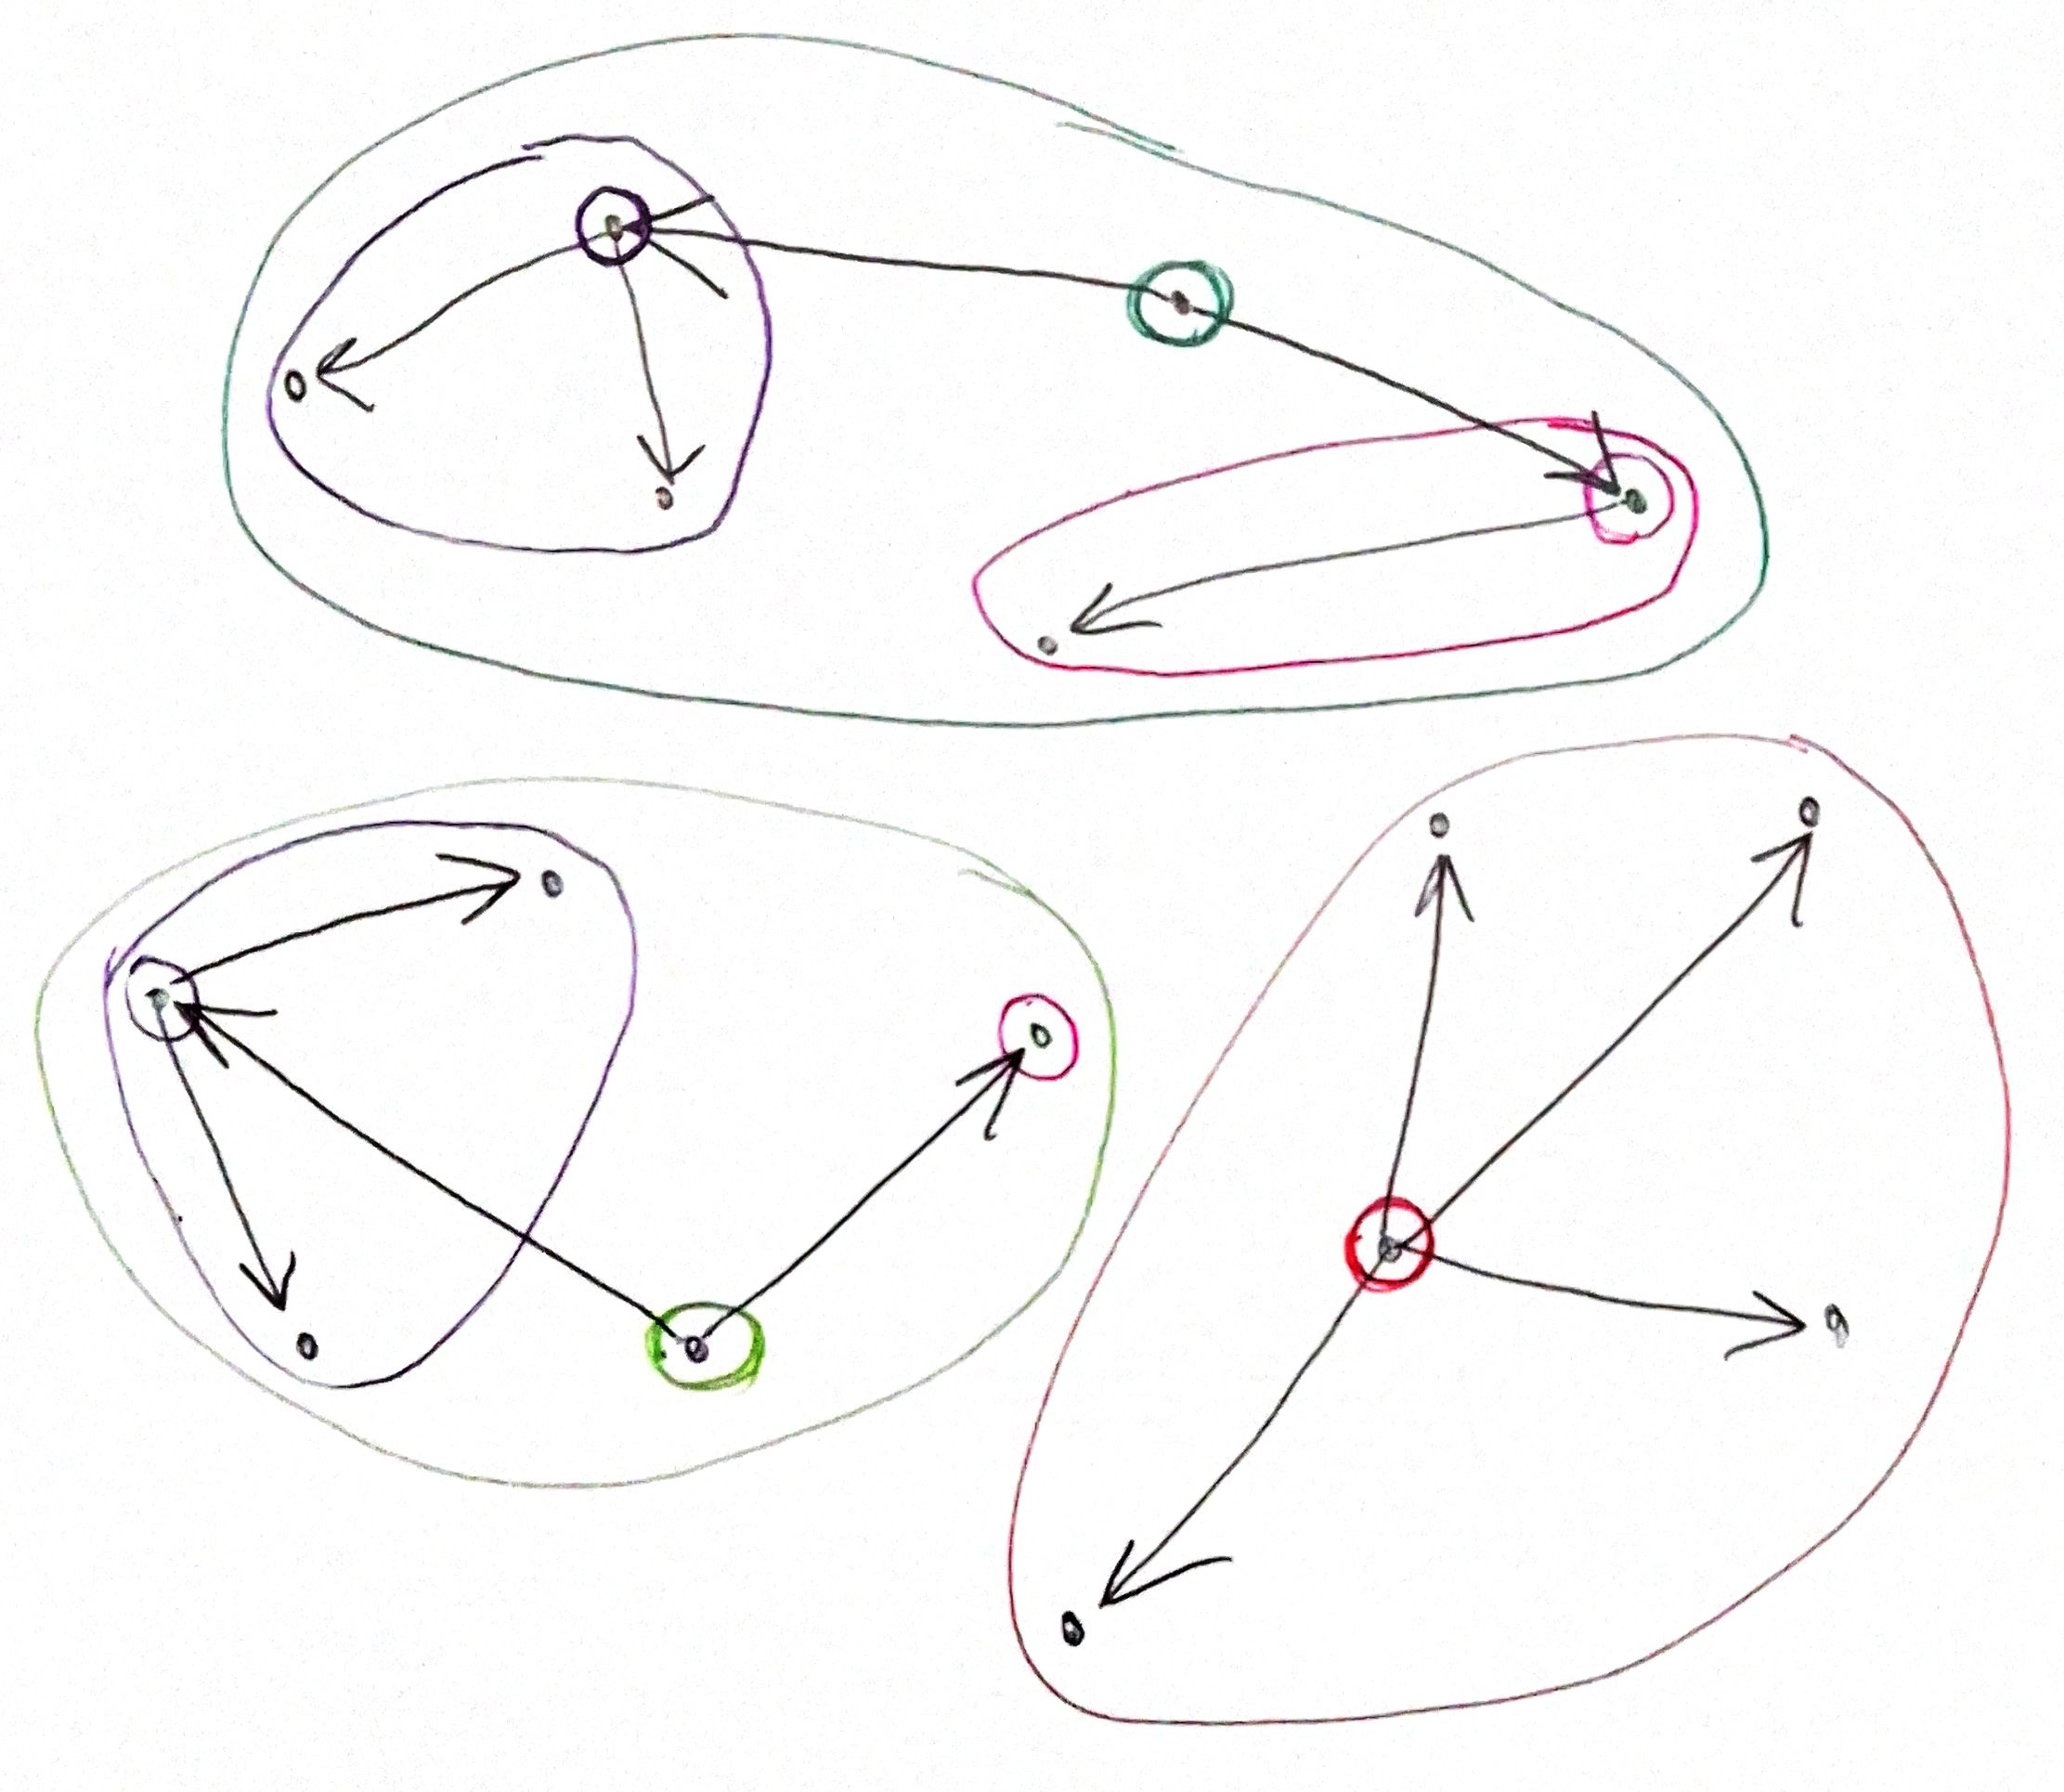
\includegraphics[width=0.5\textwidth]{images/precedence_construction.jpg}
    \caption{Precedence generation. The root nodes are the green, red and lemon. Red has four leaf vertices. Green has two branches, the pink with one leaf and the purple with two leaves. Lemon has one leaf and one branch with two leaves.}
    \label{fig:precedence-generation}
\end{figure}

\subsection{How to Generate the Weights}

Generate the weights randomly in the interval $\interval{0}{H}$.

\subsection{How to Generate the Knapsack Capacity}

Generate each entry of the knapsack capacity $\maximumWeight$ randomly in the interval $\interval{0}{m \cdot n \cdot H}$.
